\documentclass[preprint,11pt]{elsarticle}
\usepackage[T1]{fontenc}
\usepackage{float,longtable}
\usepackage[utf8]{inputenc}
\usepackage{lmodern,geometry,microtype,graphicx,booktabs,amsmath,amssymb,amsthm,tabularx,enumitem}

\usepackage[colorlinks=true,allcolors=blue,pdfauthor={Meshaal Obaid Mouawad}]{hyperref}
\geometry{margin=25mm}
\newtheorem{proposition}{Proposition}
\newcommand{\code}[1]{\texttt{#1}}
\journal{Science of Computer Programming}
\begin{document}
\begin{frontmatter}
\title{Tracing KPI Source Revisions into Version-Sensitive Governance Alert Decisions}
\author[msu]{Meshaal Obaid Mouawad\corref{cor}}
\ead{mmouawad@ece.msstate.edu}
\cortext[cor]{Corresponding author}
\address[msu]{Department of Electrical and Computer Engineering, Mississippi State University, Box 9571, Mississippi State, MS 39762, USA}
\begin{abstract}
A software revision can alter the calculation of a key performance indicator (KPI), the documentation generated from its source, or both. When an alert monitor uses a revision identity to decide whether evidence and warning deferrals remain current, these changes can produce different review decisions. We investigate the information lost when a source-to-alert interface tracks only file bytes, executable structure, or generated documentation. Nine verified source-file revision pairs from a KPI-documentation repository yield four documentation-only changes, one executable-representation-only change, two changes to both representations and two changes to neither. We map each pair to seven explicitly constructed temporal review contexts and execute four version strategies, producing 252 streams and 1,512 event decisions. Under a declared technical revalidation rule that treats either representation change as relevant, whole-file, calculation-only and documentation-only tracking differ from the dual-representation reference on 10, 20 and 5 of 63 scenario sequences, respectively. The dual strategy matches its own declared reference on all 63 sequences. All 252 strategy streams match the frozen event-policy oracle for their respective inputs. Separate proofs for that policy show that three joint version comparisons preserve displayed state, episode activity and severity; five also preserve the selected reason code. An earlier 4,935-trace benchmark independently illustrates why displayed warnings and underlying active episodes require separate evaluation. The combined evidence identifies precisely how representation choices upstream can change a downstream review decision, and which version comparisons preserve the resulting outputs.
\end{abstract}
\begin{keyword}
software evolution \sep KPI documentation \sep version-sensitive monitoring \sep provenance \sep information preservation \sep governance alerts
\end{keyword}
\end{frontmatter}


\section{Introduction}\label{sec:introduction}
The same source-code revision can have different consequences for an executable calculation and for the documentation derived from it. This distinction matters when a warning is tied to the version of the evidence that produced it: a change in documentation may require a new review even when executable structure is unchanged, and a calculation change may matter even when the generated description stays the same. We investigate how these two source-revision signals affect the version identity passed to a governance-alert monitor. The evidence combines nine actual source-file revision pairs, a reproducible mapping to a specified monitor, and formal results about which comparison signals preserve that monitor's decisions.

In enterprise reporting, a key performance indicator (KPI) such as yield, throughput or utilization is computed by code but interpreted through business-facing documentation. LEAP (Literate Programming for Automated KPI Extraction) extracts potential KPI definitions, formulas and source locations and assembles them into a browsable Interactive Bluebook \cite{mouawad2026architecture}. A source-review check can flag a record for inspection. The resulting warning may be deferred for one evidence revision; when that evidence changes, the system must decide whether the deferral still applies and whether an underlying review episode remains active. An \emph{episode} is the period during which the policy has qualified the issue for review. A \emph{displayed warning} is the state presented after applying any permitted deferral. These are separate outcomes of the version-sensitive policy studied here.

Two established research lines make the problem precise. Differential execution methods assess changes to program behavior, and code-documentation consistency methods examine divergence between source and its descriptions \cite{groninger2025changeguard,chen2024cocc}. Runtime-verification research formalizes decision-preserving input abstractions and monitoring across software versions \cite{henzinger2022abstract,guan2025imop}; warning-management research shows that suppressions can persist and hide later warnings \cite{hu2025suppressed}. The unresolved interface question addressed by this study is what follows when a single source change has \emph{two independently changing outputs} but a downstream review policy requires one current evidence identity and separately version-scoped observations and deferrals. In particular, which change distinctions alter downstream decisions, and how much version comparison information is sufficient to reproduce those decisions and their explanations?

We connect the parts through a controlled source-to-alert pipeline. Nine source pairs recovered from four Git transitions have authenticated before-and-after source snapshots. For each side we compare an executable-structure representation and LEAP-generated KPI candidate/detail fields. The resulting change flags define four alternative evidence identities: whole-file, calculation-only, documentation-only and a pair of both representations. We then supply seven explicitly constructed event histories for each pair to an unchanged review monitor. Each history provides observations, current versions, expiry times and deferral packets, so a \emph{trace} is six ordered events for one source pair under one scenario. Four strategies applied to 63 pair--scenario combinations produce 252 monitor streams. The dual-representation strategy defines the technical revalidation reference: a new context is required whenever either measured representation changes. It is an explicit study criterion rather than an externally measured correctness label.

The resulting source pairs contain four documentation-only changes, one calculation-representation-only change, two changes to both and two that change neither representation. Relative to the declared dual-output reference, whole-file, calculation-only and documentation-only strategies change complete decision sequences in 10, 20 and 5 of 63 constructed scenarios, respectively. The same frozen event-policy oracle validates every strategy's output for the version packets it actually receives. These results locate the loss at the \emph{upstream choice of revision identity}: the downstream monitor executes the same specified policy on different version packets. We also retain the prior finite-policy analysis: three joint comparisons suffice for displayed state, activity and severity, while five retain the policy's selected diagnostic reason. Its original benchmark comprises 4,935 constructed traces and 26,430 events, analyzed separately from the new source-revision study.

The study addresses three linked questions. \textbf{Q1:} Which executable-structure and generated-documentation changes occur in the recovered source pairs, and which are obscured by single-representation tracking? \textbf{Q2:} Under a specified event-policy contract, how do alternative source-version identities affect complete warning decisions and episodes across identical constructed scenarios? \textbf{Q3:} Given a chosen identity and the remaining event inputs, which compressed version comparisons preserve decisions and which also preserve reasons? Three contributions follow: (i) a traceable two-output source-revision dataset and explicit source-to-monitor mapping; (ii) a paired-strategy comparison of decision consequences against a declared technical reference; and (iii) output-specific sufficiency proofs and reproduced monitor checks connecting version representations with reviewer-facing decisions. Metadata/unit transformations and independent implementations serve as supporting conformance controls rather than separate research questions.

The following sections explain the source/documentation and monitoring research, define the review policy and source-to-alert mapping, prove the version-information results, and present the source-pair integration before the retained temporal benchmark. The Discussion compares the combined evidence with the closest predecessors and states the resulting scientific interpretation.

\section{Background and related work}
\subsection{From source-linked KPI records to review findings}

For a KPI whose implementation is spread across source code and business documentation, finding the calculation is only the beginning of review. The corresponding record must also identify where the calculation came from, how it is described, and why a reviewer might question it. LEAP reconstructs these source-linked records by discovering source files, identifying possible KPI calculations, preparing their formulas and context, attaching configured review signals, and publishing linked documentation pages in the Interactive Bluebook \cite{mouawad2026architecture}. The linked record lets a reader move from a business-facing explanation back to the evidence in code. That is the purpose of LEAP in this study; the monitor investigated here operates on its source-review findings rather than replacing the underlying extraction process.

The recovered review interface supplies a simple starting point. A rule examines text from a source artifact and produces a Boolean indication that further review may be required. A flagged result is labeled \code{REVIEW\_REQUIRED}, indicating that a source check has called for review rather than reached a final judgment. For example, the restricted-execution rule detects strings such as \code{eval} and \code{exec}; the privacy rule looks for personal-identifier strings without selected masking-related strings. These are lexical signals about source text. A token in a comment may trigger a rule without any executable violation. The observation used in the present experiment is therefore the rule's result, not an independent determination that an industrial process, a privacy law or a running program has been violated.

Table~\ref{tab:recovery} identifies the five recovered rule families used to generate those observations. Each family has a categorical severity label in the frozen study inventory. The labels are carried into a warning when the lifecycle activates it; they are not calculated from measured operational harm. One controlled source snippet is associated with one rule-family observation in an event trace. This design fixes what enters the monitor so that the later evaluation can isolate how time, revision changes and deferrals affect the decision.


\begin{table}[ht]
\centering\small
\caption{Recovered source-review predicates and their archived categorical severity labels. The evaluated predicates are lexical checks; severity labels are taken from the frozen study design inventory.}\label{tab:recovery}
\begin{tabularx}{\linewidth}{@{}>{\raggedright\arraybackslash}p{.18\linewidth}X>{\raggedright\arraybackslash\ttfamily\scriptsize}p{.32\linewidth}@{}}\toprule
Family & Source-evidence pattern & Archived severity label \\\midrule
Privacy & Personal-identifier tokens without masking/encryption-related substrings. & CRITICAL\_PRIVACY\_ALERT\\
Restricted execution & Tokens such as \code{eval}, \code{exec}, or \code{os.system}. & SECURITY\_VULNERABILITY\\
Audit completeness & Modification tokens with one or more missing audit-signature elements. & COMPLIANCE\_AUDIT\_GAP\\
Data transfer & Personal-data and movement tokens without consent/agreement tokens. & REGULATORY\_RISK\\
Lineage signing & Lineage tokens without signature-related tokens. & AUDIT\_INCOMPLETE\\\bottomrule
\end{tabularx}
\end{table}

A concrete input-to-output path makes the distinction clear. Consider a controlled Python snippet containing the text \code{eval} inside a comment. The recovered lexical check flags the snippet for review; it neither runs the code nor establishes a vulnerability. The resulting true/false finding becomes an observation associated with an evidence revision and an observation time. One positive observation does not itself create an active warning. The temporal policy developed below determines whether sufficiently persistent, current observations open an episode and whether a deferral authorized for that revision may then hide its display. This example connects the inherited source check to the new lifecycle without treating a textual match as a verified incident.

\subsection{Source evolution and generated documentation}
A changed file is not a single kind of changed evidence. Gr\"{o}ninger et al. used pairwise learning-guided execution to assess whether code transformations change program behavior, evaluating the approach on annotated source changes and transformed variants \cite{groninger2025changeguard}. Their result establishes why byte-level change detection is an imperfect substitute for behavioral comparison. Huang et al. tested consistency between code and comments before and after changes, using a feature-based approach to locate descriptions that no longer agree with code \cite{chen2024cocc}. The former targets executable behavior; the latter targets description consistency. The present source-to-alert mapping measures changes to executable structure and \emph{generated documentation output} separately, then follows the resulting version identity into another program's decisions.

Recent work in \emph{Science of Computer Programming} supplies a particularly relevant documentation perspective. Chen and colleagues examined how code-context selection affects automated parameter-description generation and reported differences across context representations \cite{chen2026context}. The same journal also presents stream-based monitoring in RTLola and partial monitoring under explicit observability and verdict conditions \cite{baumeister2026rtlola,ferrando2025partial}. Together, these studies establish that both the production of source-derived explanations and the specification of monitor outputs deserve explicit treatment. Our examined interface connects the two: a changed generated document can be relevant to review even when the chosen executable representation remains stable.

\subsection{Input information and preserved outputs}\label{sec:related-work}
The source-analysis component may know the full identifiers of an evidence revision and a policy, while the monitor receiving its events may need only the result of comparing those identifiers. To decide whether a shorter input interface is adequate, we must first ask what distinctions its output requires. If two different histories become identical after an input field is removed, any deterministic monitor receiving that reduced input must treat them alike. Its output can be correct for both histories only when the specified policy also requires the same result. This is the sense in which an input representation preserves the output. Henzinger et al. formalize this relationship for quantitative specifications by grouping observation prefixes into classes that remain equivalent under a common continuation. Each class receives one real-valued output. Their Proposition~6 bounds the difference between the two specified values by twice the permitted prompt error; exact agreement requires the values to coincide. They use these classes to relate output precision to the distinctions a monitor can retain \cite{henzinger2022abstract}. This provides the foundation for testing whether an interface merges histories that require different warnings.

Leucker et al. study a complementary representation of uncertainty: an abstract timed stream denotes the complete streams consistent with its gaps or imprecise values. Their abstract TeSSLa operators retain the precision obtainable by applying the corresponding concrete operator to those possibilities and then abstracting the results. For \code{lift}, this property requires a perfect abstraction of the underlying data function. Their analysis also shows why composing individually perfect operators can lose temporal information, and gives a time-aware construction that retains the relevant bounds \cite{leucker2019partial}. The representation and the operations applied to it jointly determine what a monitor can recover.

Jevitha et al. choose abstractions according to the property being checked. They derive finite-state models from multithreaded Java executions and reduce them using user-defined data and control abstractions. Predicate checks concern the concrete states represented by an abstract state; selected path conditions concern the connections retained between states. Their evaluation compares state counts and model-construction and verification times \cite{jevitha2024abstract}. The common question across these approaches is which distinctions the chosen output requires. In the present policy, an obsolete observation context and an obsolete observation policy can both produce an unresolved warning. A single mismatch indicator captures that decision, whereas the prescribed reason distinguishes its source.

Antignac et al. formalize a data preprocessor that preserves a program's output and give a procedure for constructing such preprocessors. Their ordering compares the input distinctions retained for a fixed output function \cite{antignac2017minimisation}. Here, the two output functions are the event decision and that decision with its prescribed reason; Propositions~\ref{prop:five-comparison} and~\ref{prop:three-comparison} establish concrete comparison encodings for the review lifecycle.

\subsection{Temporal monitoring and explanations}
Once a source finding has been converted into an observation, its meaning can change across later events. A positive finding may need to persist before a warning becomes active; a negative finding may need to persist before it clears; a deferral may expire while the review episode is still active. Runtime-monitoring methods provide the event-processing and temporal constructs needed to express such behavior. Convent et al. define transformations of timestamped streams, including delay-generated events, in TeSSLa \cite{convent2018tessla}. Baumeister et al. describe specifications over streams, derived streams and Boolean notification triggers in RTLola, with static analyses and a configurable interface to the observed system \cite{baumeister2026rtlola}. These mechanisms support the execution of a review policy after its observation and output contracts have been defined.

The event source can also determine the information available for verification. Chalupa et al.'s Vamos middleware preprocesses heterogeneous streams and represents observations lost under load through explicit gaps or summaries, such as event counts and timestamp ranges \cite{chalupa2025vamos}. Ferrando and Cardoso's partial-monitoring construction instead identifies when checking can stop or observations can be skipped because they cannot contribute to a conclusive verdict \cite{ferrando2025partial}. Both address which observations the monitor needs to process. A version-applicability comparison addresses a recorded observation whose content is available and whose authority refers to a particular evidence or policy revision.

Timing and changes to requirements add two further choices. Leucker et al. distinguish system time from event-arrival time when computing verdicts from asynchronous streams \cite{leucker2020streams}; the present evaluation specifies decisions at supplied event times. Zhou et al. analyze on/off-delay timers for stochastic anomaly detectors \cite{zhou2025delay}. Such timers determine when a condition persists long enough to change a decision. Carwehl et al. adapt runtime verification to changing requirements using timed-automata patterns and transfer relevant monitor state \cite{carwehl2023changing}. The review contract below specifies which evidence and policy changes instead reset that state.

Explaining a verdict introduces an additional output requirement. Zhang et al. use causation semantics to describe the relevance of incoming observations to an online Signal Temporal Logic verdict \cite{zhang2026caumon}. Lima et al. construct proof-tree explanations for metric first-order temporal logic and provide a verified checker; their implementation is WhyMon \cite{lima2024explainable}. The present monitor reports the contract condition selected at an event, such as an observation-policy mismatch. Its information question is whether a reduced interface retains the distinction needed to select that reason as well as the displayed decision.

\subsection{Versioned evidence and notification suppression}
A finding can qualify a review episode only when it concerns the evidence currently being reviewed under the policy currently in force. This makes provenance relevant to the decision rather than merely to its documentation. The World Wide Web Consortium provenance model (PROV), edited by Moreau and Missier, represents revision and invalidation relationships \cite{moreau2013prov}. Operational assurance systems use version information to decide which evidence supports a finding or release. Muhammad et al. combine versioned policies and schema-checked evidence bundles in a deterministic pass/warn/block gate, evaluated on 1,000 synthetic scenarios and five benchmark model configurations \cite{muhammad2026audit}. Nweke and Yeng bind runtime evidence to controls, releases, environments and timestamps, with policy or configuration digests where required. Their four-release evaluation checks provenance and evidence completeness in two identity workflows \cite{nwekeyeng2026compliance}. Open Policy Agent, used in that implementation, records the policy-bundle revision with each decision identifier \cite{opa2026logs}.

Versioned records also support temporal checking. Li et al. record model versions with threshold triggers, observation windows, metrics and proposed mitigations in a clinical audit ledger \cite{li2026sentinel}. Ra\c{t}iu et al. check temporal constraints incrementally as related engineering artifacts change, using Object Constraint Language with linear temporal operators to report process deviations over artifact histories \cite{ratiu2026runtime}. These systems connect observations or findings to the objects and versions that give them meaning.

Hinov invalidates dependent evidence when a design or its requirements change and checks replacements through an executable evidence contract. Across the constructed design cases, global abstention reproduces the final gate decisions and loses information about which constraints are unresolved \cite{hinov2026assurance}.

Suppressing a notification introduces a separate authorization. Prometheus Alertmanager stores active alerts and can mute notifications when their labels match a temporary silence \cite{prometheus2026alertmanager}. The distinction between stored activity and notification gives the review policy two relationships to check: whether the observation supports the current episode and whether the deferral applies to its warning. The constructed audit case uses that separation to expose a display error with an unchanged active interval.

Legunsen et al. monitor successive Java versions and withhold messages for violations of the same property at likely corresponding source locations \cite{legunsen2019evolution}. That filtering decision follows prior occurrence across program versions. Guan and Legunsen subsequently developed instrumentation-driven evolution-aware runtime verification: their iMOP framework reuses instrumentation for unchanged code while monitoring all specifications in new revisions. They evaluated 2,028 revisions of 66 projects with 160 monitored specifications, measuring runtime overhead and preservation of newly detected violations \cite{guan2025imop}. Jiang et al. then investigated finer-grained selection of specifications to re-monitor. Their FineMOP study compared change-impact analyses on 1,104 revisions of 68 Java projects and measured both unnecessary re-monitoring and retention of detected violations \cite{jiang2026finemop}. These studies establish revision-aware monitor selection and cost as research problems with implemented solutions. The present experiment instead keeps the monitor and its specification fixed, changes the evidence identity supplied from executable and generated-documentation representations, and measures the resulting displayed decisions and reason codes.

Hu et al. analyzed suppressed static-analysis warnings in software histories and found that some suppressions can hide subsequent warnings \cite{hu2025suppressed}. The SARIF standard already records suppression kind and review status alongside analysis results \cite{oasis2019sarif}. These are direct predecessors for the existence and representation of warning deferrals; the present experiment instead tests which upstream source-representation changes alter the version identity supplied to an explicit temporal policy. The present contribution centers on the measured connection between two source-derived representations and the version-sensitive monitor outputs.

Version-sensitive exceptions also occur in analysis tools. The \code{skill-audit} implementation binds a suppression to a fingerprint of the source, evidence, rule and scanner version; a changed fingerprint reactivates the finding. Its reports retain the finding and record the suppression separately \cite{skillaudit2026suppression}. These mechanisms establish revision-scoped exception handling. The present analysis determines which comparisons preserve the complete temporal decision and its specified reason.

Companion LEAP studies examine checks on generated KPI documentation and comparisons between source-pinned KPI definitions and their implementations \cite{mouawadjones2026checks,mouawad2026discrepancies}. Those checks supply findings about fixed source material. Here, successive revisions become inputs to a temporal policy and can change whether a finding or deferral applies. Table~\ref{tab:related-matrix} places this interface question alongside the abstractions, temporal mechanisms and versioned evidence objects established by the closest work. The following sections define the contract and establish sufficient comparisons for each output requirement.

{\small
\setlength{\tabcolsep}{4pt}
\renewcommand{\arraystretch}{1.12}
\setlength{\LTleft}{0pt}
\setlength{\LTright}{0pt}
\begin{longtable}{@{}>{\raggedright\arraybackslash}p{.235\linewidth}>{\raggedright\arraybackslash}p{.38\linewidth}>{\raggedright\arraybackslash}p{\dimexpr.385\linewidth-4\tabcolsep\relax}@{}}
\caption{Comparison of input abstractions, monitored objects, and output contracts established in the cited sources.}\label{tab:related-matrix}\\
\toprule
Approach & Input and established operation & Decision or evidential object \\
\midrule
\endfirsthead
\multicolumn{3}{l}{Table~\thetable\ (continued)}\\
\toprule
Approach & Input and established operation & Decision or evidential object \\
\midrule
\endhead
\midrule
\multicolumn{3}{r}{Continued on next page}\\
\endfoot
\bottomrule
\endlastfoot
ChangeGuard \cite{groninger2025changeguard} & Paired execution to determine whether a source revision changes executable behavior. & Behavior-change assessments for modified code. \\
CoCC \cite{chen2024cocc} & Features of code and comments before and after revisions. & Detection of outdated or inconsistent comments. \\
Parameter-description study \cite{chen2026context} & Alternative code contexts and generated parameter explanations. & Quality of generated descriptions under different contexts. \\
Suppression evolution \cite{hu2025suppressed} & Suppression histories across static analyzers and source projects. & Empirical evidence about warning suppression, including suppression of later warnings. \\
RTLola \cite{baumeister2026rtlola} & Stream specifications and asynchronous inputs; derived streams, static analyses and executable monitor construction. & Stream values and Boolean notification triggers. \\
Vamos \cite{chalupa2025vamos} & Heterogeneous event sources; preprocessing, buffering and explicit gaps or summaries when observations are lost. & Events and loss information supplied to downstream monitors. \\
Abstract TeSSLa \cite{leucker2019partial} & Timed streams with gaps or imprecise values; abstract operators and analysis of compositional precision. & Sound abstract outputs; operator-level perfection and selected perfect compositions. \\
Abstract monitors \cite{henzinger2022abstract} & Equivalence classes of observation prefixes; precision and resource requirements for quantitative monitors. & Common outputs for indistinguishable histories; bounds relating prompt error to specification-value separation. \\
Property-preserving Java models \cite{jevitha2024abstract} & User-defined data and control abstractions of execution-state models. & Preserved predicates and path conditions for runtime verification on reduced models. \\
Data minimisation \cite{antignac2017minimisation} & A program's input domains and output function; construction and comparison of output-preserving preprocessors. & The program's output with reduced input distinctions. \\
CauMon \cite{zhang2026caumon} & Signal traces and temporal requirements; online monitoring with causation semantics. & A verdict identifying the relevance of incoming observations to satisfaction or violation. \\
WhyMon \cite{lima2024explainable} & Metric first-order temporal requirements and event traces; proof-tree construction with a verified checker. & Explanations certifying satisfaction or violation. \\
Changing-requirement monitoring \cite{carwehl2023changing} & Requirement changes in self-adaptive systems; adaptation through timed-automata patterns. & Updated verification behavior with transfer of relevant monitor state. \\
Audit-as-Code \cite{muhammad2026audit} & Versioned policy and schema-checked evidence bundles; deterministic assurance gates. & Pass/warn/block decisions with policy-linked evidence. \\
Compliance-as-Code \cite{nwekeyeng2026compliance} & Control, release, environment and time-bound evidence; provenance and fixed-window completeness checks. & Evidence-linked findings and machine-readable assessment artifacts. \\
Temporal engineering compliance \cite{ratiu2026runtime} & Changes to related engineering artifacts; incremental checking of temporal constraints. & Feedback on process deviations as artifact histories evolve. \\
Evidence-grounded design assurance \cite{hinov2026assurance} & Changes to a design or its requirements; invalidation and replacement of dependent evidence. & Final gate and per-constraint verdicts, with localization not retained under global abstention. \\
Evolution-aware verification \cite{legunsen2019evolution} & Successive program versions, monitored properties and corresponding source locations. & Newly occurring violations after filtering likely repeated violation messages. \\
Instrumentation-driven evolution-aware RV \cite{guan2025imop} & Reuse of instrumentation across revisions; changed-code reinstrumentation; all specifications monitored. & Monitoring overhead and detection of new violations over 2,028 revisions in 66 projects. \\
Fine-grained evolution-aware RV \cite{jiang2026finemop} & Source-change impact analyses selecting which specifications require re-monitoring. & Monitoring cost and retained new violations over 1,104 revisions in 68 projects. \\
Alertmanager \cite{prometheus2026alertmanager} & Active alerts, label matchers and temporary silences. & Notification suppression separated from stored active alerts. \\
\code{skill-audit} \cite{skillaudit2026suppression} & Source, evidence, rule and scanner fingerprints; exact suppression matching with expiry. & Findings retained in reports with separate suppression annotations. \\
Present study & Nine recorded source revisions, paired executable/documentation representations, four alternative evidence identities and a version-sensitive event policy. & Conditional decision differences across 252 streams, an explicit reference contract, and proved output-specific comparison sufficiency. \\
\end{longtable}
}

\section{A version-bound review lifecycle}
A source check alone says whether the text examined in one artifact satisfies a configured predicate. A reviewer instead needs an event-by-event decision: has the concern persisted long enough to warrant attention, has it cleared, and is a deferral still authorized for the current version? We specify one policy that answers these questions and makes its result inspectable. The policy is the research object evaluated below, built over the recovered Boolean findings described in Section~2.1.

The policy has two linked outputs. The \emph{episode} records the concern's underlying activity after qualification, clearing and reset rules. The \emph{display} is the warning a reviewer would see after applying any valid deferral. A deferral can modify the display without changing the episode. Keeping these outputs distinct permits the evaluation to detect the obsolete-deferral error in the opening example.

\subsection{Inputs, authority and event timing}
An event is one opportunity for the monitor to update its decision. For the same source artifact and rule family, an ordered sequence of such opportunities is a trace. Each event has a review time and its unit, together with two current identities: $c$ identifies the revision of evidence relevant to the rule, and $p$ identifies the version of the review policy. These identities answer the question ``Which source evidence and which rules are authoritative now?'' Ordinary display metadata, such as a presentation label, is outside the evidence identity.

Two packets may accompany the event. An \emph{observation} contains the source check's Boolean finding (or a conflict marker), the evidence and policy versions under which it was obtained, and its timestamp. A \emph{deferral packet}, called a \emph{suppression} in the implementation, records the evidence and policy versions for which a reviewer may withhold the warning and the time at which that authorization expires. The monitor checks whether each packet refers to the current $(c,p)$ pair. A packet produced for an older version cannot acquire current authority merely because it remains stored.

The policy also specifies four durations. Qualification duration $D$ is the elapsed time between consecutive supplied positive samples required before an episode becomes active; clearing duration $C$ analogously uses successive negative samples; escalation duration $E$ governs how long an active episode may continue before its displayed urgency changes; maximum evidence age $F$ determines when an observation is stale. In the opening case the current evidence and observation name $(c_1,p_1)$, while the deferral names $(c_0,p_1)$ and expires at four seconds. The different evidence identities explain why the deferral cannot authorize suppression at the event when the warning qualifies.

Checking the observation's authority and checking the deferral's authority are different operations. The first determines whether evidence may advance the episode; the second determines whether an otherwise active warning may be hidden. Release-linked evidence contracts, revision-sensitive suppressions and label-scoped silences motivate these choices \cite{nwekeyeng2026compliance,skillaudit2026suppression,prometheus2026alertmanager}. Our controlled policy brings them together so that the consequences of accepting an obsolete packet can be measured as an actual change in the displayed decision. The proofs later cover any admissible duration settings under the specified transition order.

For the experiments, we set $D=C=F=2$ seconds and $E=4$ seconds. Reaching a qualification, clearing, escalation or freshness boundary counts as reaching the threshold; a deferral ceases to apply at its exact expiry time. Input in seconds or milliseconds is first normalized to the same unit. Required times and durations must be finite, durations must be nonnegative, and events must arrive with strictly increasing times. Malformed input causes an execution failure. These rules define the constructed lifecycle used throughout the proofs and evaluation.

Before changing an episode, the monitor checks whether the observation can be used. It must match the current evidence and policy identities, carry a Boolean value, and have an age between zero and $F$ inclusive. No observation, a conflicting value, a future timestamp, an old observation or a version mismatch makes the evidence unresolved at that event. When several faults coincide, the monitor reports the first in the following fixed order: missing observation, evidence-context mismatch, policy mismatch, future time, stale evidence, then conflict. Specifying this order lets two implementations choose the same reason even for multiply invalid packets.

Figure~\ref{fig:method-pipeline} shows how a source-review finding becomes a lifecycle decision. The interface combines that finding with the current evidence and policy identities, time, and any suppression. The monitor first applies version-change resets, then checks the observation and advances episode state, and finally determines the displayed action. This order preserves the distinction between the existence of an active episode and the warning presented at a particular event.

\begin{figure}[H]
\centering
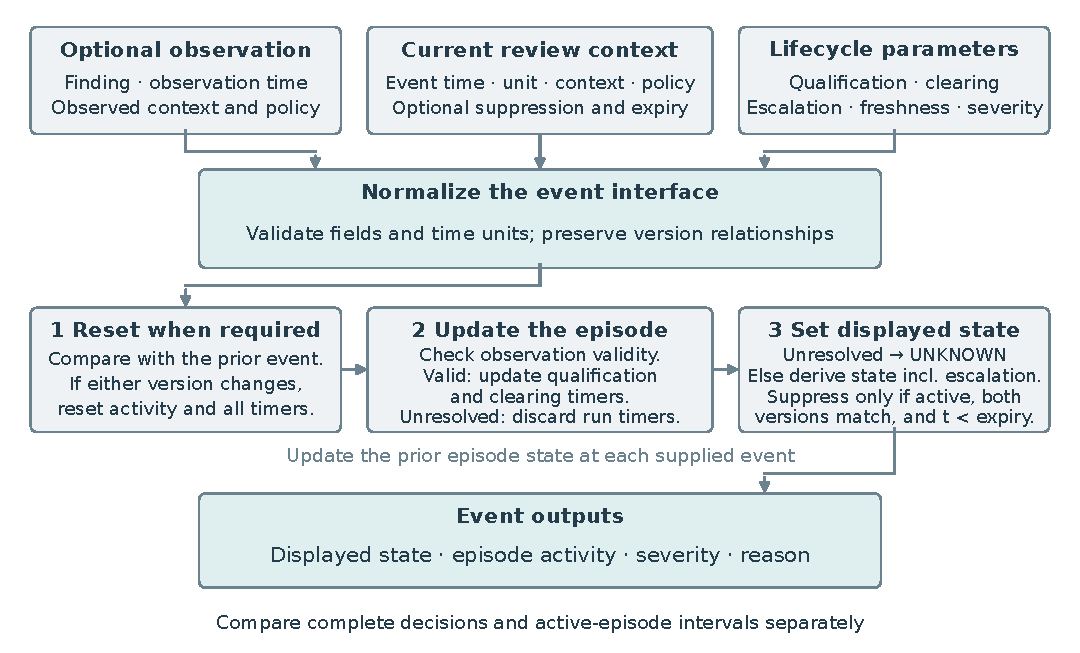
\includegraphics[width=0.88\linewidth]{method_pipeline.pdf}
\caption{Event processing under the version-bound review policy. After schema and time checks, a version change resets activity and timers. Valid observations update qualification and clearing before the monitor determines escalation and applies suppression. Unresolved observations display \code{UNKNOWN} and preserve any episode still active after the reset check. Suppression requires an active episode, matching context and policy, and event time $t$ strictly before expiry. At exact expiry the underlying episode again determines the valid display.}
\label{fig:method-pipeline}
\end{figure}

\subsection{From observations to episodes and displayed warnings}
At each event the monitor needs only its previous version pair, the start times of any positive and negative runs, the time at which an episode activated, and whether that episode is active. It first checks for a change of current evidence context or policy. Such a change resets episode activity and all timers because the previous observations no longer establish a run under the current pair.

With unchanged versions, a valid positive observation begins or continues a \emph{qualification run}. The episode becomes active at the first supplied event whose elapsed positive run reaches $D$. A valid negative observation begins or continues a \emph{clearing run}; at the first supplied event reaching $C$, the episode ends. A negative value breaks a qualification run, and a positive value breaks a clearing run. If the current observation cannot be resolved, neither run can continue, though an episode already active remains active unless the version reset has ended it. The monitor changes state only when an event is supplied; a gap between matching samples is treated as elapsed time for this sampled-event policy, without direct observation inside the gap. Passage of wall-clock time, including deferral expiry, does not produce a separate decision until a new event is supplied.

After these episode updates, the monitor decides what the reviewer sees. A valid episode still active at the first event at least $E$ seconds after activation is displayed as \code{ESCALATED}. If a valid, active episode also has an unexpired deferral matching the current evidence and policy, the display becomes \code{SUPPRESSED} instead. Suppression does not clear the episode or stop its activation clock; when the authorization expires, the underlying episode again determines the display. An unresolved observation displays \code{UNKNOWN}, even if the monitor retains an earlier active episode.

The other displayed states are \code{CLEAR}, \code{PENDING}, and \code{ACTIVE}. Each output contains three components: the state displayed to the reviewer, a Boolean flag recording underlying episode activity, and a severity label. The active severity comes from the applicable rule family in Table~\ref{tab:recovery}; escalated severity is HIGH. Suppressed and inactive displays have severity NONE, and unresolved displays have severity UNKNOWN. A fourth field, the reason, names the condition that selected the output. The separation of these four fields is what permits the later experiments to compare an invisible episode error with a visible warning error.

\paragraph{Concurrent conditions and the reported reason}
The transition order and the reason-selection order are specified separately. Each event names one current context and one current policy. A change in either first resets episode activity and all timers. If both change, the reset label is \code{POLICY\_CHANGE}; a context-only change gives \code{CONTEXT\_CHANGE}. Observation validation then selects the first applicable condition in the ordered list \code{MISSING}, \code{CONTEXT\_MISMATCH}, \code{POLICY\_MISMATCH}, \code{FUTURE}, \code{STALE}, \code{CONFLICT}. A malformed packet fails schema validation before these decisions are produced.

At event index $i$, let $q_i$ be the selected observation-validity label, or empty for valid evidence, and let $R_i$ be the selected reset-reason label, or empty when no reset occurs. Let $d_i$ denote the displayed state after the state update and suppression overlay. The reported reason is
\begin{equation}
\operatorname{reason}_i=
\begin{cases}
q_i, & q_i\ne\varnothing,\\
R_i, & q_i=\varnothing\ \land\ R_i\ne\varnothing,\\
\text{SUPPRESSION}, & q_i=R_i=\varnothing\ \land\ d_i=\text{SUPPRESSED},\\
\text{STATE}, & \text{otherwise},
\end{cases}
\end{equation}
The selected validity label takes diagnostic precedence even though a simultaneous version reset has already changed the underlying episode state. For example, a current-policy change with an observation still bound to the previous policy produces \code{UNKNOWN}, inactive activity and reason \code{POLICY\_MISMATCH}. If both observation bindings mismatch, the reason is \code{CONTEXT\_MISMATCH}. If matching evidence is both stale and conflicting, the reason is \code{STALE}.

For valid evidence, timer updates determine activity before escalation and suppression are displayed. Clearing at its boundary yields \code{CLEAR} even when escalation would otherwise become due at that event. Valid suppression overlays an active or escalated display while retaining the activation clock. At exact suppression expiry, the overlay ends. Unresolved evidence displays \code{UNKNOWN} with its validity reason, including when a valid suppression is present. When a valid reset and suppression coincide with immediate activation under zero qualification duration, the displayed state is \code{SUPPRESSED} and the reason is the reset label.

The evaluation includes a separately frozen set of concurrent-condition cases to check this priority across four implementations.

\section{From source revisions to monitoring contexts}\label{sec:source-bridge}
The temporal policy requires a current evidence identity $c$; a software repository supplies source revisions, not this identity directly. We make the upstream mapping inspectable by distinguishing two source-derived representations. For an archived source version $v$, let $R_C(v)$ be a deterministic executable-structure representation and $R_D(v)$ be the LEAP-generated KPI candidate and detail fields. The corresponding signatures $h_C(v)$ and $h_D(v)$ are SHA-256 hashes of these representations. A changed signature establishes a change in the measured \emph{representation}. It is not a claim of behavioral inequivalence on every possible program input or of independently verified documentation meaning.

For a before/after revision $(v_0,v_1)$, define $\Delta_C=[h_C(v_0)\ne h_C(v_1)]$ and $\Delta_D=[h_D(v_0)\ne h_D(v_1)]$. The experimental revalidation criterion is $\Delta_{\mathrm{ref}}=\Delta_C\lor\Delta_D$: either measured output change makes the evidence context new. This criterion supplies a precise reference against which competing mappings can be compared. A whole-file strategy $A$ uses a source-byte hash, calculation strategy $B$ uses $h_C$, documentation strategy $C$ uses $h_D$, and dual strategy $D$ uses the ordered pair $(h_C,h_D)$. They are evaluated on the \emph{same} archived revision and the same event history; only the current evidence identity and its associated observation/deferral bindings differ.

Table~\ref{tab:revision-pairs} gives the recovered distribution. The nine source pairs come from four Git commit transitions; each before/after snapshot has a verified source hash. Four revisions change only generated documentation, one only executable structure, two both and two neither. In particular, a whole-file identity changes on all nine revisions even though the two measured output representations are stable for two of them. The distinction makes both over-resetting and omitted revalidation observable within the declared criterion.

\begin{table}[ht]
\centering\small
\caption{Actual source revisions classified by changes in two measured representations. Each row denotes an archived source-file pair, not an independently collected organizational event. The categories are determined from the supplied deterministic signatures.}\label{tab:revision-pairs}
\begin{tabularx}{\linewidth}{@{}lcc>{\raggedright\arraybackslash}X@{}}\toprule
Case IDs & $\Delta_C$ & $\Delta_D$ & Measured revision class\\\midrule
P7R03, P7R07 & 1 & 1 & Both representations change\\
P7R09 & 1 & 0 & Executable representation only\\
P7R01, P7R02, P7R04, P7R05 & 0 & 1 & Generated documentation only\\
P7R06, P7R08 & 0 & 0 & Neither measured representation changes\\\bottomrule
\end{tabularx}
\end{table}

The integration then constructs seven fixed monitoring histories per source pair. All start with the prior source version at times 0 and 2 seconds and introduce the new version from the event at 3 seconds. Events continue at 5, 7 and 9 seconds. The scenarios exercise a fresh positive finding, a fresh negative finding, an observation bound to the earlier evidence revision, an earlier deferral with expiry, missing observations, a policy change, and an observation bound to the old policy after that change. Each supplies explicit Boolean findings and packet timestamps; no finding or deferral is inferred from the source edit itself. Four evidence-identity strategies applied to $9\times7=63$ paired contexts produce $4\times63=252$ streams, or 1,512 event decisions.

The reference monitors use the existing frozen event-policy oracle. The \emph{identity-mapping} reference is separately defined by the dual criterion $\Delta_{\mathrm{ref}}$: this separates the question ``Did the monitor execute the policy for its inputs?'' from ``Did the upstream identity retain the two change signals the experimental objective requires?'' A zero difference for the dual strategy is expected from its construction; scientific interpretation therefore turns on the mismatches of alternative inputs and the source pairs that cause them. The old benchmark still tests monitor execution using its own 4,935 constructed traces. The new integration tests the boundary between source revision analysis and that unchanged monitor.

\section{What information must the monitor retain?}\label{sec:information}
The policy above uses version identifiers for a narrowly defined purpose: it checks whether the current evidence and policy have changed and whether an observation or deferral names those current versions. This suggests that a separate source-analysis component might pass the results of those checks to the monitor rather than pass the identifiers themselves. The scientific question is whether those comparison results contain enough information for the specified outputs.

Consider two otherwise identical events with valid, active episodes and unexpired deferrals. One deferral names the current revision and must hide the warning; the other names an obsolete revision and must leave the warning visible. Removing the deferral's version field without supplying a match indicator makes the events indistinguishable, even though the required displayed states differ. The following propositions first formalize when such information loss is fatal and then show how a small set of Boolean comparisons can preserve the outputs.

A \emph{projection} is the input left after an upstream transformation deletes or merges selected fields. The relevant question is whether every pair of histories mapped to the same projected input also demands the same output. Proposition~1 applies the standard indistinguishability principle to histories grouped by a fixed input projection. Henzinger et al. give its quantitative counterpart for abstract monitors in Proposition~6 \cite{henzinger2022abstract}. Proposition~2 is the empirical form of the maximum-posterior decision rule under zero--one loss. For a trace drawn uniformly from the benchmark multiset, the normalized bound is the maximum probability of recovering the required sequence after observing the whole projected trace \cite[Definition~3]{smith2009foundations}. Propositions~\ref{prop:six-comparison}--\ref{prop:three-comparison} establish sufficient encodings for the specified policy and distinguish preservation of decisions from preservation of their reasons.

Let $X$ be the set of admissible complete traces, $Y$ the set of decision sequences, and $Z$ the set of projected traces. The function $G:X\rightarrow Y$ returns the reference sequence of displayed states, activity flags, and severity labels. The projection $P:X\rightarrow Z$ removes a specified field. A deterministic monitor restricted to this interface computes $M:Z\rightarrow Y$. Policy parameters and all remaining side inputs are included in $Z$.

\begin{proposition}[Indistinguishable evidence]
If $P(x_1)=P(x_2)$ and $G(x_1)\ne G(x_2)$, no deterministic function of the projected input is correct on both traces.
\end{proposition}
\begin{proof}
The two equal projected inputs produce one output under $M$. That output cannot equal two different required decision sequences.
\end{proof}

\begin{proposition}[Finite-benchmark bound]
For a finite multiset of $N$ traces, let $n(z,y)$ count traces with projected input $z$ and reference sequence $y$. Every deterministic function of that projection has at most
\begin{equation}
B(P)=\sum_z\max_y n(z,y)
\end{equation}
correct complete traces.
\end{proposition}
\begin{proof}
Within each projection class, the function returns one sequence and can match at most the largest reference-sequence group. Summation over disjoint projection classes gives the bound. A full-trace lookup function can attain it by choosing a most frequent label in each class. The same bound applies to causal monitors.
\end{proof}

The first proposition establishes an impossibility condition: if the reduced representation makes two differently answered traces identical, no downstream algorithm can repair the missing distinction. The second proposition counts, for a fixed finite benchmark, the maximum number of complete traces any algorithm using that representation could classify correctly. This is a bound on what the input permits, not an accuracy estimate for an independently sampled industrial population.

Figure~\ref{fig:witness} illustrates a constructed observation-context witness. The two traces differ only in the observation's context after the first event. Current context, current policy, Boolean values, and times are equal. Removing the observation-context field makes the remaining inputs identical; one reference sequence activates and the other remains unresolved. A corresponding suppression witness distinguishes \code{ACTIVE} from \code{SUPPRESSED}, with activity retained in both cases.

\begin{figure}[H]
\centering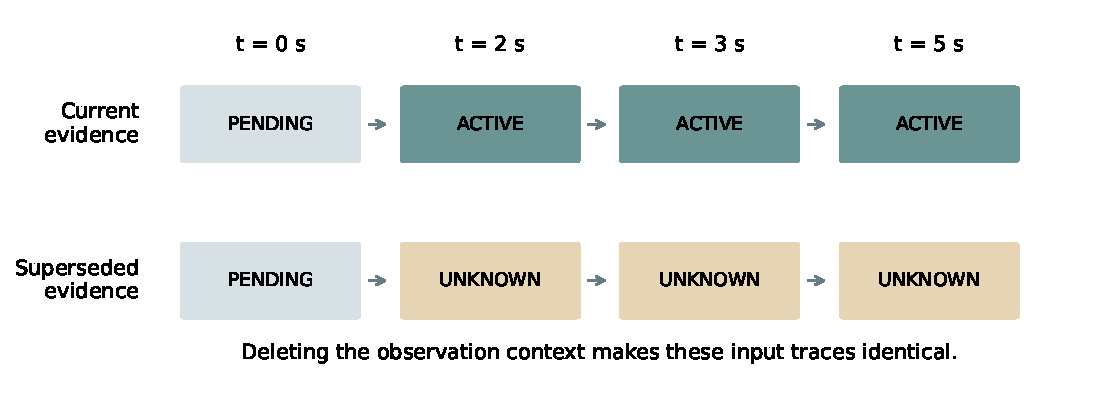
\includegraphics[width=\linewidth]{necessity_witness.pdf}
\caption{A constructed observation-context witness. Boxes show the required displayed state at successive supplied events, equally spaced by event order. Both observations match the current context at 0\,s. From 2\,s onward only the upper row matches, so qualification produces \code{ACTIVE} there while the lower row displays \code{UNKNOWN}. Removing the observation-context field makes the remaining inputs identical.}\label{fig:witness}
\end{figure}

The witness construction repeats this test for six individual identities: the current evidence context and policy, the evidence context and policy named by the observation, and the evidence context and policy named by the deferral. Each projection has one pair per rule family. Trace identifiers and intervention labels are excluded from the monitor interface. The analytical witness assay fixes base severity to High; six structural pairs are instantiated under five rule identifiers. The performance benchmark uses each recovered severity string. These inherited strings are categorical labels; HIGH escalation is a study-defined label, with no empirically ranked severity claim. The witness assay retains full inputs, canonical projected inputs, their hashes, and both reference sequences. It evaluates necessary information for this policy independently of the choice of implementation algorithm.

\begin{proposition}[Sufficiency of version comparisons]\label{prop:six-comparison}
For an admissible trace, the raw version names can be replaced by six Boolean comparisons per event: whether the current context and policy each changed since the preceding event, whether an observation's context and policy each match the current event, and whether a suppression's context and policy each match. The observation and suppression comparisons are defined when their respective packets are present. Given the remaining inputs, these comparisons suffice for the displayed decision, activity, severity, and reason at every event.
\end{proposition}
\begin{proof}
Initialize both change indicators to false. Suppose two encoded prefixes agree through event $i$ and have identical timers and activity at its start. The two change indicators determine the reset and its reason. The observation comparisons, time, and value determine validity and hence the same timer update. The suppression comparisons and expiry give the same displayed state. Activity, severity, and reason then agree, as do the timers for the next event. The common initial state establishes the induction.
\end{proof}
The induction shows why the monitor does not need the original version names once these comparisons are supplied: each update depends on whether the version changed or matched, not on the identifier's spelling. The six comparisons are sufficient but retain one distinction that the specified reason rule never outputs. In particular, the reason \code{SUPPRESSION} is selected only after an applicable suppression actually changes the display. An inapplicable suppression does not produce separate context-mismatch or policy-mismatch reasons.

\begin{proposition}[Five-comparison sufficiency for decisions and reasons]\label{prop:five-comparison}
For every admissible trace, the complete sequence of displayed states, activity flags, severity labels and specified reasons is determined by the retained non-version inputs and at most five Boolean comparisons per event:
\[
(\Delta^c_i,\Delta^p_i,O^c_i,O^p_i,S^{\mathrm{joint}}_i).
\]
Here $\Delta^c_i$ and $\Delta^p_i$ indicate changes in the current evidence context and policy version since the preceding event (both false initially); $O^c_i$ and $O^p_i$ indicate matches of the observation's two version fields when present; and $S^{\mathrm{joint}}_i$ is true exactly when a present suppression matches both current versions. Packet presence, observation values, event and observation times, expiry, policy durations and rule severity remain available.
\end{proposition}
\begin{proof}
Induct on the event index. The two current-change indicators uniquely select the reset and its reason, including policy precedence when both change. For a present observation, $O^c_i$ and $O^p_i$ select the applicable context- or policy-mismatch reason in the specified order. All other validity checks use retained values and times. Consequently, the timer and episode transitions agree. The suppression overlay depends only on the episode's active status, the retained expiry and $S^{\mathrm{joint}}_i$. The reason rule selects an observation-validity label first, then a reset label, then \code{SUPPRESSION} only if the overlay is displayed, and otherwise \code{STATE}. It never outputs which suppression field mismatched. Therefore the two separate suppression comparisons can be replaced by their conjunction without changing any of the four output components. The updated timers and activity provide the induction hypothesis for the next event.
\end{proof}
The five-comparison result identifies a practical interface contract. The evidence-producing component must distinguish an observation's context mismatch from its policy mismatch, because those can produce different reported reasons. For a deferral, it need report only whether both bindings match, because the policy reports \code{SUPPRESSION} when suppression actually takes effect and does not give separate reasons for unsuccessful deferral matches. This sharpens the six-comparison result without claiming a globally minimal encoding. A receiving component that reports decisions but not reasons needs still fewer distinctions. 

\paragraph{An interface for decisions alone}
The following encoding uses $\Delta_i$ as a Boolean change indicator. Let $k_i=(c_i,p_i)$ denote the current evidence-context and policy pair at event $i$. Let $\Delta_i$ indicate that $k_i$ differs from $k_{i-1}$, with $\Delta_1=0$. Let $v_i$ and $m_i$ indicate respectively that the observation and suppression, when present, name $k_i$. Presence, observation value, timestamps and expiry remain inputs. At most three Boolean comparisons therefore accompany each event.
\begin{proposition}\label{prop:three-comparison}
The triple $(\Delta_i,v_i,m_i)$ suffices for the sequence of displayed state, activity, and severity under the stated policy. It need not determine the reported reason.
\end{proposition}
\begin{proof}
The monitor resets when $\Delta_i$ is true. For a present observation, either kind of version mismatch clears the qualification and clearing runs and produces the same unresolved display; $v_i$ distinguishes that case from a matching observation. Given valid evidence and an active episode, a present deferral overrides the display exactly when $m_i$ holds and the expiry time is later than the event time. All other transitions use the retained time and value fields. Induction from the common initial state gives identical activity, display, and severity at each step. For the reason field, consider two otherwise identical first events with positive observations: one names an obsolete context under the current policy and the other names the current context under an obsolete policy. Both give $v_1=0$ and the same unresolved decision. The specified reasons are context mismatch and policy mismatch, respectively.
\end{proof}

\section{Evaluation design}
The evaluation has two distinct evidence layers. First, archived source revisions establish how executable and generated-documentation representations change; the new paired event histories test the effect of the resulting version identities. Second, the previously frozen temporal benchmark tests the policy and its input abstractions across a broader constructed set of event histories. These layers use different experimental units and references. The source study answers Q1, its 252 streams answer Q2, and the proofs and representation checks answer Q3. Supplementary ablations and invariance checks address the contract's boundary conditions. No source-revision case is counted as a newly observed organizational alert history.

\subsection{Benchmark and split}
The benchmark begins with five source-rule families (Table~\ref{tab:recovery}). For each family, the recovered adapter examines positive and negative controlled snippets and produces Boolean findings. The archive links those findings to the original snippets, their hashes and the adapter provenance. A separate generator then constructs event sequences by assigning times, evidence and policy identities, evidence-quality conditions and deferrals to the findings. The lifecycle monitor receives these temporal packets; it does not execute the source snippets. Source-rule fixtures check the upstream predicates, while the newly constructed event traces test the downstream monitoring contract.

The generator covers both routine and adversarial event histories. Short combinations of positive, negative, missing and conflicting observations test the basic state changes; longer controls exercise sustained conditions; interventions deliberately alter evidence quality, revision identity or deferral applicability; boundary designs test the exact time at which a decision should change. For each rule family, the frozen generator defines 329 base designs: $4^4=256$ length-four sequences over positive, negative, conflicting and missing observations; three length-twelve controls; $11\times5=55$ intervention designs; and $5\times3=15$ temporal-boundary designs. The length-four sequences have event times $0,2,4,6$\,s. The controls comprise twelve negative observations, twelve positive observations, and an activation--clearing sequence whose values at $t=0,\ldots,11$\,s are one negative, seven positive and four negative observations.

Every intervention starts from that activation--clearing control. Each of the eleven operations in Table~\ref{tab:intervention-taxonomy} is applied at each index $j\in\{2,3,5,7,9\}$, yielding exactly 55 designs per family. Here the zero-based index equals event time in seconds. A single intervention means one selected operation: the four evidence-quality operations change one event, whereas version changes and suppression assignments affect the indicated suffix. The supplementary grid lists all 55 type--position pairs and their frozen trace identifiers.

\begin{table}[H]
\centering\small
\caption{Complete intervention taxonomy. Each row contributes five base designs per rule family, one at each intervention index. The ordinary context and policy are $c_1,p_1$; $c_0,p_0$ denote nonmatching identities and $c_2,p_2$ revised identities.}
\label{tab:intervention-taxonomy}
\begin{tabularx}{\linewidth}{@{}>{\raggedright\arraybackslash}p{0.26\linewidth}>{\raggedright\arraybackslash}X>{\raggedright\arraybackslash}p{0.12\linewidth}@{}}
\toprule
Operation & Exact modification & Extent \\
\midrule
Missing observation & Remove the observation packet at index $j$. & Event $j$ \\
Conflicting observation & Set its finding value to null. & Event $j$ \\
Stale observation & Set observation time to $j-3$\,s, giving age $3>F$. & Event $j$ \\
Future observation & Set observation time to $j+1$\,s. & Event $j$ \\
Revised context, old evidence & Set current context to $c_2$ and retain observation context $c_1$. & $i\ge j$ \\
Revised policy, old evidence & Set current policy to $p_2$ and retain observation policy $p_1$. & $i\ge j$ \\
Revised context, fresh evidence & Set both current and observation context to $c_2$. & $i\ge j$ \\
Revised policy, fresh evidence & Set both current and observation policy to $p_2$. & $i\ge j$ \\
Matching suppression & Attach suppression for $(c_1,p_1)$, expiring at $j+2$\,s. & $i\ge j$ \\
Old-context suppression & Attach suppression for $(c_0,p_1)$, expiring at $j+2$\,s. & $i\ge j$ \\
Old-policy suppression & Attach suppression for $(c_1,p_0)$, expiring at $j+2$\,s. & $i\ge j$ \\
\bottomrule
\end{tabularx}
\end{table}

The fifteen boundary designs test qualification, clearing, escalation, freshness and suppression at offsets $-0.5$, $0$ and $+0.5$\,s from the relevant boundary. They contain respectively two, four, three, two and three events per design. Suppression packets remain present after expiry in their intervention suffixes, allowing the policy to evaluate expiry explicitly.

We also test whether changes to representation that leave policy meaning unchanged alter a decision. Each base design has three representations: its original form, a variant with irrelevant display metadata added to every event, and an equivalent millisecond representation scaling event times, observation times and suppression expiry by 1,000. Across five families, the corpus therefore contains 1,645 design groups and $329\times3\times5=4,935$ traces. The four design categories contribute, respectively, 3,840, 45, 825 and 225 traces, comprising 15,360, 540, 9,900 and 630 events; the total is 26,430 events. The taxonomy audit compares the policy-input fields of every intervention representation with the frozen records after time-unit normalization.


Development and held-out comparisons use different source-rule families so that the scored families were not used to tune the study implementation. The partition is by source-rule family. Privacy and restricted execution supply the 658 development base traces. Audit, transfer, and lineage supply 987 held-out base traces and 5,286 events, with 2,961 traces and 15,858 events after the two transformations. Simulated source identifiers and rule families are disjoint across the partition, and the three representations of each family-design group remain together. All five families instantiate the same 329 temporal templates. The source predicates supply Boolean inputs upstream, and the temporal evaluation checks contract conformance across these family instances. The sample size follows finite mechanism coverage.

\subsection{Reference and verification protocol}
To measure agreement, the study needs an expected decision independent of the tested monitor's code. A separate AI review agent therefore implemented a reference directly from the written policy without viewing the incremental monitor. The reference reconstructs decisions from prefixes and contiguous valid observation runs. Before benchmark scoring, 29 hand-derived cases specified transitions, exact boundaries, invalid evidence, suppression and malformed inputs. The specification, implementations, analysis script, inputs and reference outputs were frozen before the held-out comparison; the manifest records their identities and freeze time.

Post-evaluation verification uses a separately versioned validation reference that requires an explicit time-unit field during schema validation. The archive retains this reference and the original one. Their outputs are compared on the complete benchmark and witness set. Twenty-eight malformed-input probes check the schema, while 24 hand-calculated concurrent-condition traces check the precedence rules in the review contract. The concurrent-case inputs and expectations were frozen before execution and scored in the full incremental monitor, the validation reference, SQLite and PyContract. They contain 75 events per implementation and are analyzed separately from the original benchmark.

OpenAI ChatGPT and Codex assisted with source recovery, implementation, reference construction, experiment orchestration, and analysis. Deterministic programs produced every scored decision, and the retained inputs and programs support replay of those decisions.

Figure~\ref{fig:mismatches} plots complete-decision and active-episode mismatches from saved outputs for the 987 held-out base traces. Its underlying counts are recomputed from archived event-level decisions. Editable figure source and reproduction steps are supplied with the research materials.

\subsection{Comparisons and outcomes}
The primary endpoint is stricter than agreement about whether an issue was active. It asks whether a monitor produces the same displayed state, activity flag and severity at every event in an entire trace. A trace fails that endpoint if even one displayed decision differs. We also score active-episode intervals independently, because a hidden warning can leave those intervals unchanged. The original offline evaluation ran under Python 3.12.14 on Linux x86-64. Each method received the same ordered packets, time-unit declarations, base severity and policy. The base-only analysis gives each of the 987 designs equal weight. To reproduce the primary endpoint, let $a_{ij}$ and $g_{ij}$ denote the output and reference decision tuples at event $j$ of trace $i$. For trace length $n_i$ and $N$ traces, exact-trace agreement is
\[
N_{\mathrm{exact}}=\sum_{i=1}^{N}\prod_{j=1}^{n_i}\mathbf{1}[a_{ij}=g_{ij}].
\]
The product is one only when every event in a trace agrees; the sum counts such traces. A single event disagreement therefore changes a complete trace's score.
The full monitor and independent retrospective reference implement the same contract. Four reduced implementations isolate different requirements: timer-only processing removes version resets and observation/suppression binding; no-evidence-binding preserves resets and timing but accepts obsolete observation versions; no-suppression-binding accepts suppressions from other versions; no-freshness removes the stale-age check while retaining rejection of future-dated observations. Every method receives identical events, policy parameters, and recovered severity. A snapshot comparator directly reports the inherited Boolean finding at each event, separately characterizing the difference between snapshot and lifecycle interfaces.

Primary agreement requires equality of every $(\text{state},\text{active},\text{severity})$ tuple in the complete trace. Event agreement uses that same tuple. Missed active decisions have reference activity true and output activity false; unwarranted active decisions reverse those values. Episode agreement compares the entire list of half-open active event-index intervals, ending at trace length for an open final episode. Severity and policy-reason agreement are separately counted. Execution failures and unresolved states are retained in the record. The fixed corpus is fully enumerated, so the endpoints are exact descriptive counts with explicit denominators. The primary analysis counts each base design once.

\subsection{Additional implementation and fixture checks}
These checks followed the primary evaluation and use separately frozen protocols. The SQL and PyContract implementations receive the original corpus, policy parameters and categorical family severities. They test execution of the same contract through different computational representations.

\paragraph{Recursive SQL implementation}
The SQL implementation expresses the complete policy as a recursive query in SQLite 3.53.1. Python validates and loads the inputs and compares the outputs; SQLite computes the transitions. The query, driver, reference hashes and analysis addendum were frozen before this implementation was scored.

\paragraph{Established monitoring engine}
A retrospective comparison encoded the complete experimental policy in PyContract, a runtime-verification library introduced by Dams et al. for event streams and parameterized state machines \cite{dams2022pycontract,pyrv2025pycontract}. The executed upstream snapshot was pinned to commit \texttt{e378eed38699bcff33e2ae71426e6b161690cdfa}; its source files were verified against Git blob hashes. The policy specification used four data states: Dormant for an inactive episode without a qualification run, Qualifying for an inactive episode with a positive run, Raised for an active episode outside clearing, and Recovering for an active episode in a clearing run. Guards check evidence quality, version changes, freshness and suppression. The unmodified PyContract engine dispatched each event and maintained the active state vector. The specification imported neither the proposed monitor nor the reference oracle.

The baseline protocol, encoding, upstream source, inputs and references were frozen before scored execution. Per-event logging records calls to the upstream dispatcher. An integration check temporarily disables each of three upstream dispatch methods, then restores it, to verify that the imported engine participates in producing the output.

\paragraph{Externally specified suppression outcomes}
A supplementary conformance check used expected suppression outcomes from the versioned Alertmanager test suite. The first four \code{Mutes} assertions in \code{TestSilencer}, version 0.28.1, specify the outcomes for an absent silence, a nonmatching exact matcher, a matching exact matcher, and an expired silence \cite{prometheusSilencer0281}. We froze their source lines, expected Boolean outcomes, and mapping before replay. The retained source has verified Git blob \code{a65b1f6337723d3ba76140081b757088213f7d5a}; the supplement includes its Apache 2.0 license and content hashes.

The adapter mapped exact equality of the source test's \code{foo} label to equality of the review-policy context, with a fixed matching policy version. Two positive observations established an active episode before each query, and the source test's relative expiration time was preserved. Where the source retained both a matching and a nonmatching silence, the fixed-label projection retained the matching candidate. The mapped output was whether the final displayed state was \code{SUPPRESSED}. This extension was frozen separately after the primary experiment.
The study implementations execute the mapped inputs, and the scored endpoint is the externally specified suppression Boolean.

\section{Results}
\subsection{Recorded revisions distinguish calculation and documentation change}\label{sec:revision-results}
Across the nine archived before/after source pairs, signatures of executable structure changed in three cases, and generated-documentation fields changed in six. Their overlap comprises two cases. Four documentation-only revisions would be treated as unchanged by calculation-only tracking; the single calculation-only revision would be treated as unchanged by documentation-only tracking. Two revisions modify source bytes without changing either measured representation. These categories are directly recoverable from the recorded source snapshots and extractor outputs in Table~\ref{tab:revision-pairs}.

Runtime checks are a separate measurement. Seven of the nine pairs have comparable execution fixtures: five yielded equal recorded execution outputs, while two yielded a different execution status or output. One of the two differences is a transition from an unresolved variable to a successful calculation; a SQL fragment has unresolved input bindings, and an ABAP example lacks an available runtime. Accordingly, the $3/9$ executable-structure count measures a source representation rather than a universal numerical-behavior difference. The source pairs establish a real divergence in what the two representations record, not the correctness of any review authorization.

\subsection{Effect of the source-to-alert mapping}\label{sec:bridge-results}
For each source pair, the seven constructed histories were evaluated under whole-file ($A$), executable-structure ($B$), generated-documentation ($C$), and dual-representation ($D$) identities. Every strategy received the same findings, times, policy version and packet pattern. Table~\ref{tab:bridge-results} reports discrepancies against the specified dual-representation revalidation reference. The denominator for complete traces is 63 per strategy (nine pairs times seven scenarios); for event fields it is 378 per strategy (63 traces times six events).

\begin{table}[ht]
\centering\small
\caption{New source-to-alert integration, relative to the declared dual-representation technical reference. ``Missed'' counts a pair whose measured representation changed but the strategy retained its previous identity; ``extra'' counts an identity change when neither measured representation changed. Complete-sequence differences compare the state/activity/severity tuple at every event. The reference row's zero differences follow from the chosen criterion.}\label{tab:bridge-results}
\begin{tabular}{@{}lrrrr@{}}\toprule
Version identity & Extra resets / 2 & Missed changes / 7 & Differing / 63 & Equal / 63\\\midrule
$A$: whole file & 2 & 0 & 10 & 53\\
$B$: executable structure & 0 & 4 & 20 & 43\\
$C$: generated documentation & 0 & 1 & 5 & 58\\
$D$: paired representations & 0 & 0 & 0 & 63\\\bottomrule
\end{tabular}
\end{table}

The observed differences have a direct causal path \emph{within the specified model}: the strategy selects a different evidence identity at the revision boundary; the policy then processes an observation or deferral using that identity. A documentation-only revision such as P7R02 is invisible to calculation-only identity $B$ even though it changes the dual context. In the constructed old-observation scenario at three seconds, $B$ reports reason \code{STATE}, while $D$ reports \code{CONTEXT\_MISMATCH}. The source and monitoring inputs for that exact pair are included in the archived comparison packets. Conversely, P7R06 changes file bytes without changing either representation: its fresh-positive scenario reports \code{CONTEXT\_CHANGE} under $A$ where $D$ reports \code{STATE}. These are precise examples of a missed version distinction and an additional version reset, respectively; the displayed reason can differ even when another summary metric is unchanged.


Table~\ref{tab:source-bridge-witness} follows the complete six-event P7R02 old-observation input, rather than selecting only the first differing event. The archived source revision leaves the executable representation unchanged but changes the generated-documentation representation. The scenario then supplies an observation carrying the earlier evidence identity at every event after the revision at $t=3$ seconds. Strategy $B$ retains the old executable identity and therefore continues the episode; $D$ sees the documentary change, treats those observations as context-mismatched, and leaves the episode inactive. The reference for this comparison is the explicitly selected dual-output revalidation contract.

\begin{table}[ht]
\centering\small
\caption{Complete recorded output for the constructed P7R02 old-observation scenario (six events). $B$ tracks only the unchanged executable representation; $D$ also detects the generated-documentation change at 3 seconds. Values and reasons are transcribed from the frozen integration file \code{decision\_events.csv}; activity is 1 for active and 0 otherwise. \code{CM} abbreviates \code{CONTEXT\_MISMATCH} and \code{ST} abbreviates \code{STATE}.}\label{tab:source-bridge-witness}
\begin{tabular}{@{}rlrllrl@{}}\toprule
$t$ (s) & $B$ display & $B$ activity & $B$ reason & $D$ display & $D$ activity & $D$ reason \\\midrule
0 & PENDING & 0 & ST & PENDING & 0 & ST \\
2 & ACTIVE & 1 & ST & ACTIVE & 1 & ST \\
3 & ACTIVE & 1 & ST & UNKNOWN & 0 & CM \\
5 & ACTIVE & 1 & ST & UNKNOWN & 0 & CM \\
7 & ESCALATED & 1 & ST & UNKNOWN & 0 & CM \\
9 & ESCALATED & 1 & ST & UNKNOWN & 0 & CM \\\bottomrule
\end{tabular}
\end{table}

Differences are visible in every reported field. Relative to $D$, strategy $A$ changes displayed state on 20 of 378 events, episode activity on 22, severity on 18 and reason on 18. The corresponding counts for $B$ are 40, 44, 36 and 36; for $C$ they are 10, 11, 9 and 9. All four strategies produce the same complete decision sequence in 28 of the 63 contexts. Thus different revision identities do not always imply different displayed sequences: the policy's observation validity, timer state, packet presence and event time determine whether a lost distinction is visible at a specific event.

All 252 streams and 1,512 event tuples matched the unchanged frozen event-policy oracle for their respective supplied inputs. This establishes conformance of downstream policy execution for the integration packets, separately from the choice of source identity. The exact comparison is retained in the recorded machine-readable event outputs and can be reproduced by the same integration command.

\subsection{Preserving decision outputs and diagnostic reasons}\label{sec:bridge-representations}
Each of the 252 streams was additionally projected into the three-, five- and six-comparison interfaces of Section~\ref{sec:information}. The three-comparison decoder reproduced displayed state, activity and severity on all 252 streams and 1,512 events. It preserved reason sequences on 180/252 streams; 180 of 1,512 event reasons differed from the full interface. The five- and six-comparison encodings reproduced all four output fields on all streams and events. These are tests of output-specific information preservation applied to the integrated packet histories. They do not add independent source revisions or change the original proof obligations.

\subsection{Frozen temporal-policy results as a separate validation layer}

The experiments reveal two different failures when a monitor loses version information. An obsolete observation can change whether the underlying episode qualifies, whereas an obsolete deferral can change only what is displayed. We report the information-loss witnesses first, then compare complete decision sequences with active episodes and evaluate invariance and implementation checks.

\subsection{Version information and output requirements}
The paired histories show why individual version fields cannot simply be deleted: two histories that then look identical can require different displays. For each of the six projections, deleting one field without supplying its comparison prevented exact agreement on at least one member of every tested pair. All 30 frozen pairs had equal projected inputs and different required decisions. For each of the six projections, ten traces formed five heterogeneous classes, giving $B=5$ and an agreement upper bound of $5/10$ on that projection's assay. A supplementary generic class-count audit reproduced these bounds from canonical projected inputs and verified that the incremental monitor agreed with all 60 witness reference sequences. Each projection is a separate interface experiment.

The results distinguish two kinds of information loss. Observation-version loss permits an obsolete positive finding to influence a new episode. Suppression-version loss permits an obsolete deferral to hide a current warning. The second effect is invisible to a metric that compares only latent activity. Current context and current policy identities also have witnesses: their omission makes it impossible to distinguish an unchanged episode from an episode that must be reset under the specified policy.

\paragraph{Effect of merging the reason categories}
For a retrospective implementation check of the original six separate comparisons, we recoded each version as an alternating token on change and each nonmatching packet field as a reserved token. Across all 4,935 frozen traces, replay reproduced every reference sequence, including its reasons. This replay uses the original monitor and examines a representation property separately from the held-out implementation comparison. A post-review five-comparison canonicalization check uses the same frozen packets, changes only the version representation, and separately compares decisions and reasons with the retained reference; it is reported with the supplement rather than counted in the original evaluation.
In a retrospective replay we encoded the three joint comparisons, representing all changes as context changes and all mismatches as context mismatches. All 26,430 decision tuples in 4,935 traces matched the frozen reference. Of the 585 reason differences, 510 were policy mismatches recorded as context mismatches and 75 were policy changes recorded as context changes. These are counts for this explicit decoding. The paired example above establishes why a different decoder still cannot recover both reasons in general.

\subsection{Complete decisions and active episodes}
\label{sec:agreements}
A monitor that detects the correct episode can still make the wrong reviewer-facing decision. The clearest example is the suppressed warning: when the deferral's version binding is ignored, the active episode remains correct but the warning can be hidden. We compare these two outputs separately rather than summarize them with one agreement statistic. The complete monitor matched the reference on all 2,961 held-out traces and all 15,858 event tuples. Table~\ref{tab:results} separates complete-decision agreement from active-episode agreement and active-event errors for the 987 base designs. Metadata and time-unit variants are excluded from this table so each base design contributes once. All six compared implementations completed every trace without execution failures. The reference contains 1,803 unresolved decisions among 5,286 base events; these represent specified missing, conflicting, or invalid evidence states.

\begin{table}[H]
\centering\small
\caption{Held-out base designs: 987 traces and 5,286 events. Trace agreement compares state, activity, and severity. Missed/unwarranted counts concern active-event decisions. Reference-active denominator: 1,293; reference-inactive denominator: 3,993.}\label{tab:results}
\begin{tabular}{@{}lrrrr@{}}\toprule
Method & Trace agreement & Episode agreement & Missed & Unwarranted\\\midrule
Version-bound &987&987&0&0\\
Timer-only &897&927&0&192\\
No evidence binding &957&969&0&84\\
No suppression binding &957&987&0&0\\
No freshness &969&975&6&18\\
Snapshot comparator &246&246&408&1,179\\\bottomrule
\end{tabular}
\end{table}

Timer-only processing disagreed on 90 of 987 base traces and produced 192 unwarranted active decisions. Across all held-out variants these become 270 trace mismatches and 576 unwarranted active decisions. Observation-binding removal caused 30 base-trace mismatches and 84 unwarranted active events. Removing the stale-age check caused 18 base-trace mismatches, six missed active events, and 18 unwarranted active events. This ablation therefore produced errors in both directions of active-event classification.

Suppression-binding removal caused 30 base-trace mismatches and 48 event-tuple mismatches, while all 987 active-episode interval sequences remained correct. Every discrepancy in this ablation concerned displayed state and severity; the active-episode endpoint registered none of them. Figure~\ref{fig:mismatches} compares the mismatched base-trace counts for the complete and reduced lifecycle implementations.

\begin{figure}[H]
\centering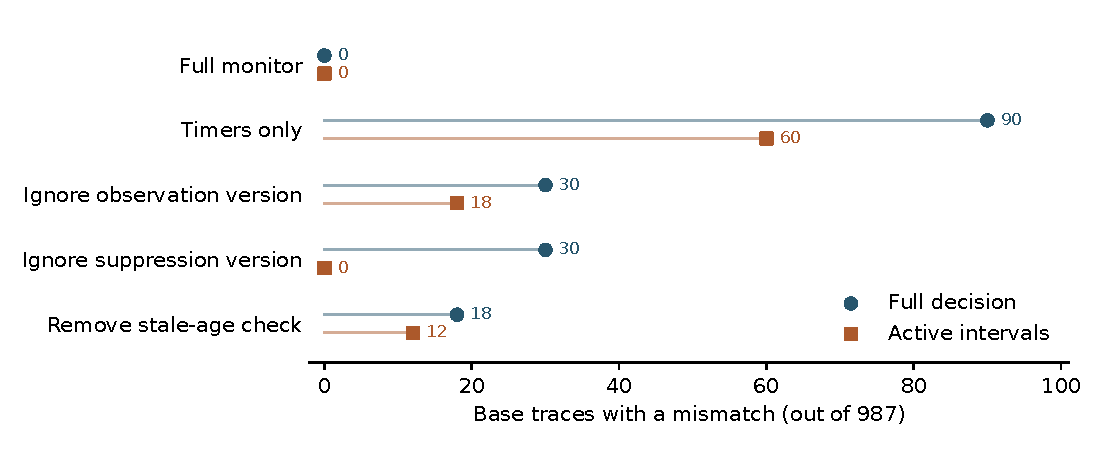
\includegraphics[width=\linewidth]{trace_mismatches.pdf}
\caption{Complete-decision and active-interval mismatches across the same 987 held-out base traces. Circles count traces with a differing sequence of displayed state, activity or severity. Squares count traces with differing lists of active intervals. Removing suppression binding changes complete decision sequences on 30 traces, with all active intervals preserved.}\label{fig:mismatches}
\end{figure}

Table~\ref{tab:attributes} counts discrepancies on the same 5,286 base events. Severity describes the warning shown at an event. The reason code identifies the policy condition that selected it.
\begin{table}[H]
\centering\small
\caption{Attribute discrepancies across 5,286 events in the 987 held-out base traces. The decision tuple contains state, activity and severity. The snapshot comparator uses a single snapshot-specific reason code.}\label{tab:attributes}
\begin{tabular}{@{}lrrr@{}}\toprule
Method & Decision tuple & Severity label & Reason code\\\midrule
Version-bound & 0 & 0 & 0\\
Timer-only & 342 & 342 & 282\\
No evidence binding & 204 & 204 & 204\\
No suppression binding & 48 & 48 & 48\\
No freshness & 51 & 51 & 18\\
Snapshot comparator & 1,851 & 1,761 & 5,286\\
\bottomrule
\end{tabular}
\end{table}
The full monitor's reason and severity fields also matched the reference on all 15,858 held-out events. Reason agreement identifies the same contract condition as the reference at each event. The snapshot comparator agreed on 246 base traces, reflecting the differences between immediate Boolean reporting and the study's qualification, clearing, suppression, and revision policy. All detailed results, including mechanism and family strata, are derived from the saved per-event outputs.

\subsection{Invariance under metadata and unit changes}
A change of presentation label or an equivalent representation of time should not count as a new finding, policy, or deferral. The transformations test whether an implementation changes its behavior when only those irrelevant representations change. Each method produced identical complete outputs for all 3,290 base-to-transformed comparisons across the full benchmark: 1,645 metadata comparisons and 1,645 time-unit comparisons. This invariance held for the complete monitor, all four reduced implementations, and the snapshot comparator. The transformation checks therefore passed even for methods with mismatched reference decisions.

\subsection{Reference and concurrent-condition checks}
The principal benchmark assumes the source predicates and the event-policy reference are the intended inputs. Additional checks examine that assumption directly: the recovered source rules must produce the expected family identifiers, the intervention records must match their declared changes, and simultaneous conditions must follow the prescribed precedence. Replaying eleven archived source fixtures reproduced the expected rule identifiers in all eleven cases. The taxonomy audit matched the policy-input fields of all 825 intervention representations against the frozen records after time-unit normalization. These checks connect the source adapters and described intervention grid to the inputs used in the temporal evaluation.

The incremental monitor and original reference agreed on all 1,974 development traces. The validation reference rejected all 28 malformed-input probes and preserved every original benchmark and witness output. The post-evaluation corrected-reference regressions comprised 21 valid traces and eight malformed inputs, and all 29 passed.

The full incremental monitor, the validation reference, SQLite and PyContract each matched every expected final decision and reason in the 24 concurrent-condition cases: 96/96 implementation--case checks passed. Their full output sequences also agreed across all 75 events per implementation. The checks include coincident version resets and invalid observations, clearing and escalation boundaries, and suppression at exact expiry.

\subsection{Execution in SQLite and PyContract}
Agreement between the incremental monitor and its reference is strengthened when the same policy can be implemented through different computational mechanisms. We therefore encoded the specification in recursive SQL and in an established event-monitoring library, then compared both against the retained reference. SQLite reproduced all 26,430 event decisions, severities and reasons on the same 4,935 traces, with zero execution failures. It matched all 60 witness sequences and passed 21 hand-trace and 28 malformed-input checks.

The PyContract implementation received all 4,935 original traces, comprising 26,430 events, with identical policies and categorical family severities. It matched the frozen reference on \textbf{4,935/4,935 complete traces} and \textbf{26,430/26,430 event tuples}; reason, severity and active-episode intervals also agreed exactly. It recorded zero missed active decisions among 6,465 reference-active events, zero unwarranted active decisions among 19,965 reference-inactive events, and zero execution failures. The original development and held-out subsets, retrospectively replayed, yielded 1,974/1,974 and 2,961/2,961 matching traces, respectively. Separate checks passed on 60/60 witness sides, 21/21 hand-calculated valid traces and 28/28 malformed-input cases.

Per-trace records confirm 26,430 calls through the upstream PyContract event dispatcher and the corresponding data-state transitions. Disabling each of the three checked dispatch methods caused the integration check to fail; restoring the methods restored the expected output.

\subsection{Projected suppression fixtures}
The external suppression check asks a narrow question: when a silence is absent, nonmatching, matching or expired, does the mapped review policy make the same Boolean suppression decision? It therefore tests the authority-and-expiry part of the lifecycle against a separately specified set of expectations. All four mapped outputs reproduced the externally specified suppression expectations: false for an absent silence, false for a nonmatching exact matcher, true for a matching exact matcher, and false for an expired silence. Complete output sequences also agreed with the reference, all four episode-activation checks passed, and no execution failed.

\section{Discussion}
The integrated finding concerns the \emph{interface between a changing source artifact and a version-bound decision policy}. A file hash, executable-structure signature and generated-documentation signature identify different equivalence classes of source revisions. Because the policy uses an evidence identity to reset episodes and reject obsolete packets, choosing one of these classes changes the inputs against which observations and deferrals are checked. The nine archived source pairs establish the presence of both documentation-only and executable-only changes; the conditional monitor histories show exactly when those missed or additional identity changes propagate into warning decisions. This is the contribution of the combination, rather than any one signature or monitor transition considered alone.

The result sits between established research on change validation, documentation and warning lifecycle. ChangeGuard examines whether code revisions preserve executable behavior \cite{groninger2025changeguard}; code-comment consistency research examines whether descriptions remain aligned with changed code \cite{chen2024cocc}. Hu et al. show from software histories that suppressed warnings can remain and may affect later warnings \cite{hu2025suppressed}. The evolution-aware iMOP and FineMOP studies optimize which code and specifications need repeated verification as programs change \cite{guan2025imop,jiang2026finemop}. SARIF provides a standardized representation for suppression status \cite{oasis2019sarif}. For the review-policy contract in this paper, the question is more specific: when source-derived executable and documentary representations supply the evidence identity, which changes in that identity alter the displayed warning and its reason? The nine source revisions and controlled event histories support this source-to-decision relation under the declared revalidation criterion.

The formal results give the interface question a second dimension. Henzinger et al. develop the general relationship between indistinguishable histories and monitor outputs \cite{henzinger2022abstract}; the propositions in Section~\ref{sec:information} specialize that principle to this policy's version applicability, displayed warning and diagnostic reason. A producer can transmit three joint comparison results to retain the policy's decision tuple or five comparisons to retain its reason distinctions. The new integration tests these representations on every constructed stream without modifying the established policy. This distinction between \emph{which source features define a version} and \emph{which comparisons of those versions the monitor must retain} is the organizing result of the paper.

The original ablation also explains why the endpoint must include the displayed warning. In the frozen 987 held-out base traces, removing deferral applicability changed 30 complete decision sequences and 48 event tuples while preserving all 987 active-episode intervals. The effect is determined by the policy's separation of episode activity from suppression, a separation already present in operational notification systems \cite{prometheus2026alertmanager}. Its scientific role here is to show why an episode-only scoring measure is insufficient for the specified decision contract. The independent SQLite and PyContract implementations establish repeatability of that contract; they do not supply evidence about the frequency of such failures in deployment.

Taken together, the measurements define a reproducible test pattern for future source-linked review systems. First identify the concrete source representations that matter to the review objective. Then define which changes invalidate a current evidence context, construct or recover event histories, and compare complete decisions as well as reason labels. The observed counts also show why apparent performance of the reference cannot itself justify the criterion: dual tracking has zero reference disagreements by construction, and the actual comparative information resides in the archived source-change distribution and the alternate identities' differing outputs. The Limitations section specifies the evidence boundary for interpretation and reuse.

\section{Conclusion}
A source revision can alter a KPI's executable structure and its generated documentary record independently. In nine recorded revision pairs, four changed only documentation, one changed only executable structure, two changed both, and two changed neither representation. When these pairs were connected to an unchanged version-sensitive review policy through seven specified event histories each, whole-file, calculation-only and documentation-only identities differed from the declared dual-output decision reference on 10, 20 and 5 of 63 complete sequences. The result exposes concrete information lost by each representation choice and the downstream decisions affected under the policy.

For that same contract, three joint comparisons preserve displayed state, activity and severity; five also preserve the selected reason code. The 252-stream integration reproduced these output properties and retained the earlier 4,935-trace formal-monitor evaluation separately. The contribution is an inspectable source-to-alert mapping that joins paired source-representation changes with output-specific monitor information requirements, providing a bounded account of when evidence identity matters to review decisions.

\section{Limitations}
The nine archived revision pairs come from four Git transitions in one repository. Their executable signatures represent Python abstract syntax or SQL/ABAP token screens; their documentation signatures represent the selected deterministic LEAP output fields. Neither representation is an exhaustive semantic equivalence check. Seven cases have comparable execution fixtures, and the reported executable output changes apply to those fixed inputs. One SQL fragment has unresolved input bindings and the ABAP case lacks a runtime. The four strategy differences measure identity selection against the explicitly declared dual-representation revalidation criterion; that criterion is a study objective, not an externally validated organizational rule.

The 63 integrated event histories are constructed from seven temporal scenarios for each source pair. Actual alert, deferral and policy histories were unavailable for all nine pairs; findings, packet versions, times and expiry conditions were supplied for controlled sensitivity analysis. Their 252 strategy streams are correlated by pair and scenario, and the reported denominators are descriptive rather than population estimates. A dual-representation mapping matches its reference by construction. The upstream source classes and policy version identities are inputs to the model, and a different review objective could require different equivalence criteria.

The earlier lifecycle policy and its 329 temporal templates per rule family are constructed research materials. Its 4,935 traces repeat those templates across families and representation transformations. The policy uses elapsed time between matching supplied samples; no decision is emitted between events, including at a deferral-expiry instant without a subsequent event. Findings are lexical source-review signals rather than validated defects. The reference and monitor implementations share the written policy; cross-implementation agreement checks conformance to that contract, not effectiveness on deployed review processes.

The version-comparison propositions establish sufficiency for the specified policy, retained timing/value inputs and chosen output fields. They instantiate general abstraction principles already developed in formal-monitoring research. The external suppression check covers four pinned silence cases through a fixed-label projection, rather than executing the full upstream notification program. Generalization to additional source repositories, unseen temporal requirements, recorded review decisions, and wider alert-management systems remains unmeasured.

\section*{Research materials}
The accompanying reproduction archive and the preserved source-to-alert integration addendum contain the nine before/after revision pairs, two-representation signature comparisons, constructed integration inputs, 252 strategy streams, decision-event outputs and an executable preservation manifest, alongside the frozen temporal packets and reference sequences, monitor implementations, pinned third-party source and licenses, raw outputs, and analysis scripts. From its extracted \code{Paper7\_Reproduction} directory, run \code{python -B run\_all.py ../paper7-run}. The command verifies the preserved package, replays the frozen study, independently rescores the raw outputs, and runs the intervention-taxonomy and concurrent-condition checks. The added review checks have their own manifest. From the preserved integration root, run \code{python -B verify\_preservation.py} followed by \code{python -B integration/run\_integration.py}; the resulting \code{integration/outputs/RESULTS.md} records all new denominators and strategy-level decisions. The source-provenance inventory identifies the original adapters and their archived versions. Editable figures, the original renderer metadata (Matplotlib 3.10.8), figure-verification code, and the literature-discovery records accompany the manuscript.

\section*{Declaration of generative AI and AI-assisted technologies in the manuscript preparation process}
During preparation of this work, the author used OpenAI ChatGPT and Codex for manuscript drafting, editorial review, and figure preparation and verification code. The author takes responsibility for the content of the article.

\renewcommand{\bibfont}{\small}
\bibliographystyle{unsrtnat}
\bibliography{Paper7_References}
\end{document}
